\chapter{Iteración 4}

\begin{quotation}[Computer Scientist]{Donald Knuth (1938--)}
Premature optimization is the root of all evil.
\end{quotation}

\begin{abstract}
Esta iteración se orienta a mejorar la interacción del usuario con el sistema a través de
la interfaz y la presentación visual. Se consolidan el \textit{Head-Up Display}, el menú
de pausa y el menú principal del juego, y se actualizan los sprites y prefabs para aportar
una estética más propia al proyecto.
\end{abstract}

\section{Análisis de características}
La cuarta iteración se orientó principalmente a mejorar la experiencia de uso del sistema
fuera del combate y de la exploración estricta. Hasta este punto, el proyecto ya disponía
de una base jugable relativamente sólida, con generación procedural, progresión por
círculos, dualidad del jugador y una primera versión del minimapa. Sin embargo, la
interacción con el juego seguía siendo todavía pobre desde el punto de vista de interfaz,
flujo de entrada y salida, y personalidad visual. Por ello, esta iteración se centró en
cuatro funcionalidades: el ajuste del \textit{Head-Up Display}, la incorporación del menú
de pausa, la consolidación del menú principal y la actualización de sprites y prefabs.

\begin{enumerate}
\item \textbf{Head-Up Display.} Esta funcionalidad se centró en mejorar la legibilidad y el
encaje visual de la información en pantalla. En esta fase, el HUD ya existía como soporte
de ciertos elementos informativos del juego, pero todavía necesitaba una mejor adaptación al
espacio visible para resultar realmente útil durante la partida. El trabajo realizado en
esta iteración consistió en ajustar el tamaño y la disposición de los elementos visibles del
HUD para que su lectura fuera más clara y para que no compitieran de forma incómoda con el
espacio de juego. En términos funcionales, esta feature no introduce una nueva capa de
información, sino que refina la forma en la que el jugador recibe la información existente,
mejorando la proporción, el equilibrio visual y la integración de la interfaz sobre la
escena. Esto era importante porque, a medida que el proyecto iba incorporando más sistemas,
la interfaz dejaba de ser un añadido accesorio y pasaba a convertirse en una herramienta
necesaria para que el estado del juego se percibiera con claridad.

\item \textbf{Menú de Pausa.} Esta funcionalidad incorporó un flujo de interrupción controlada
dentro de la partida. Su comportamiento real consistió en detener temporalmente la
ejecución del juego, ocultar el HUD cuando correspondía, ofrecer acciones de reanudación,
reinicio y salida, y responder tanto a teclado como a mandos. La feature fue importante
porque convirtió la pausa en un estado explícito del sistema y no en una simple pantalla
superpuesta, permitiendo que el jugador pudiera interrumpir y retomar la sesión de forma
predecible.

\item \textbf{Menú Principal.} Esta funcionalidad consolidó la pantalla de entrada al
juego, responsable de cargar la escena principal y organizar las acciones iniciales del
sistema. Además de permitir iniciar la partida y salir de la aplicación, durante la
iteración se realizaron ajustes de disposición para que el logotipo y los botones se
adaptaran mejor al espacio disponible. Con ello, el proyecto dejó de depender de un
arranque puramente técnico desde la escena jugable y pasó a ofrecer una entrada más propia
de un producto interactivo completo.

\item \textbf{Actualizar Sprites.} Esta funcionalidad se centró en reforzar la identidad
visual del juego mediante la incorporación de nuevos sprites diseñados para el proyecto y
la actualización de prefabs que dependían de esos recursos. Su alcance no se planteó como
un sistema nuevo de diseño o implementación, sino como una sustitución y ajuste de recursos
para que personajes, elementos de interfaz y objetos principales encajaran mejor con una
estética propia. El objetivo era que la presentación dejara de apoyarse en una apariencia
provisional y empezara a transmitir una identidad visual más reconocible.

\end{enumerate}

La combinación de estas funcionalidades hizo que esta iteración actuara como una fase de
maduración de la capa de presentación. Aunque no se centró en añadir profundidad al núcleo
de combate o generación, sí resultó clave para mejorar la relación entre el jugador y el
sistema, ordenando mejor la información, estructurando la navegación entre estados del
juego y reforzando la identidad visual del proyecto.

\section{Diseño}
El diseño de esta iteración partió de una necesidad clara: el juego ya no podía seguir
tratando la interfaz como un elemento secundario. A medida que el sistema crecía, resultaba
necesario distinguir mejor entre la experiencia puramente jugable y la experiencia de
interacción global con la aplicación.

\subsection{Diseño de Head-Up Display}
La decisión principal respecto al HUD fue asumir que su valor no depende solo de la
información que muestra, sino también de cómo se integra visualmente con la escena. Un HUD
mal proporcionado puede ser tan problemático como la ausencia de información, ya que invade
espacio de juego o dificulta la lectura rápida del estado actual de la partida.

Por ello, el trabajo de diseño en esta iteración se centró en el ajuste de escala y
proporciones, buscando que los elementos visibles mantuvieran presencia suficiente para ser
útiles, pero sin romper el equilibrio del encuadre. La intención no era rediseñar por
completo la interfaz, sino llevarla a un punto en el que pudiera convivir mejor con el
resto del sistema.

\subsection{Diseño de Menú de Pausa}
El menú de pausa se concibió como una capa superpuesta que interrumpe temporalmente la
ejecución del juego sin romper el estado de la sesión. Esta decisión exigía una relación
directa con el control del tiempo, del audio y de la visibilidad de la interfaz de
gameplay, ya que pausar la partida debía afectar al comportamiento del sistema y no solo a
la presencia de una ventana en pantalla.

También se tuvo en cuenta que el menú debía funcionar correctamente con distintos métodos
de entrada. Por ello, su diseño priorizó acciones claras y un flujo reducido: reanudar,
reiniciar o salir, evitando introducir opciones accesorias que pudieran complicar una capa
destinada a interrumpir la partida de forma rápida.

\subsection{Diseño de Menú Principal}
El menú principal se diseñó como puerta de acceso al sistema, centralizando el inicio de
partida y la salida de la aplicación. A diferencia del menú de pausa, no depende del estado
de una sesión en curso, sino que actúa como punto de entrada anterior al bucle jugable.

Además, se decidió prestar atención a la disposición adaptable de los elementos, especialmente
del logotipo y de los botones, para evitar una composición rígida o mal proporcionada entre
distintas pantallas.

La actualización de sprites no se trató como un bloque independiente de diseño, sino como
una mejora de recursos aplicada sobre la estética general. La decisión relevante fue
integrar los nuevos sprites en los prefabs existentes para que la identidad visual avanzara
sin introducir una arquitectura nueva.

\section{Implementación}
La implementación de esta iteración se apoyó menos en nuevos sistemas lógicos profundos y
más en controladores de interfaz y ajustes de escena. Aun así, el trabajo realizado no fue
meramente cosmético, ya que varios de los cambios introducen comportamiento funcional
directo sobre el flujo del juego.

\subsection{Implementación de Head-Up Display}
La feature de HUD se materializó principalmente mediante ajustes sobre la escena de juego,
modificando el tamaño de los elementos de interfaz ya presentes para mejorar su legibilidad
durante la partida. Aunque esta intervención no requirió la creación de un gran controlador
nuevo, sí tuvo un efecto funcional claro: mejorar la forma en la que el jugador percibe la
información ya disponible.

Este tipo de refinamiento es relevante en un proyecto de videojuego porque la utilidad del
HUD depende tanto de su contenido como de su presencia visual. Con este ajuste, la interfaz
de partida quedó mejor adaptada al espacio real de uso y más preparada para convivir con
otras capas de información que se incorporarán en iteraciones posteriores.

\begin{figure}[htbp]
\begin{center}
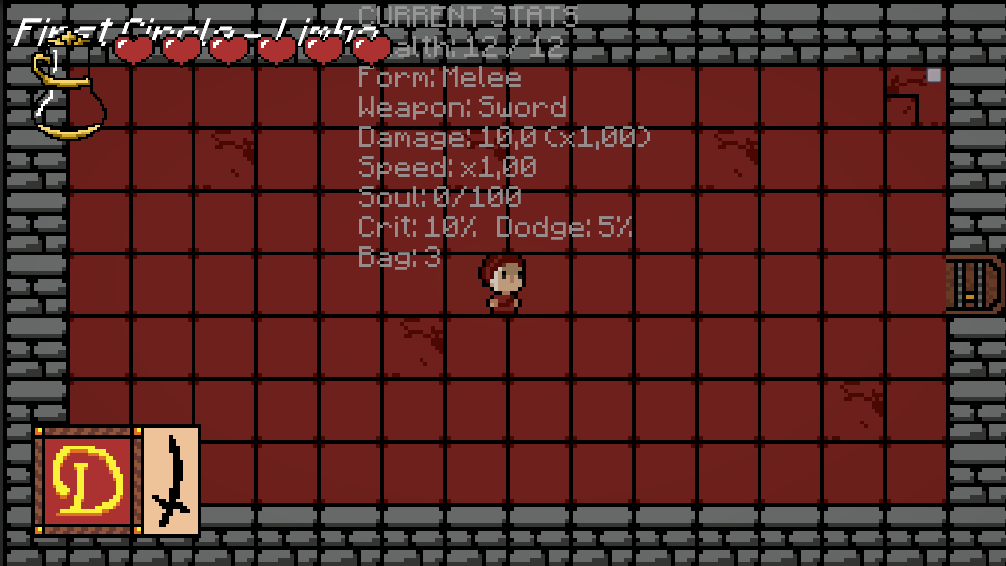
\includegraphics[width=.9\textwidth]{figures/resultados/iteracion4/10_HUD.png}
\caption{Resultado de la feature Head-Up Display en la iteración 4}
\label{fig:iteracion4-feature-hud}
\end{center}
\end{figure}

\subsection{Implementación de Menú de Pausa}
La implementación del menú de pausa se apoyó en \texttt{PauseMenuController}. Este script
controla el ciclo de pausa dentro de la partida, escuchando la entrada correspondiente,
alternando el estado pausado, ocultando o mostrando la interfaz de juego y gestionando las
acciones de reanudar, reiniciar y abandonar la sesión.

Desde el punto de vista funcional, la lógica de pausa tiene varias consecuencias directas:
detiene el tiempo mediante \texttt{Time.timeScale}, pausa el audio global, selecciona el
botón adecuado para facilitar la navegación y restaura el estado normal al reanudar. De
esta manera, el menú de pausa deja de ser una simple pantalla visual y pasa a convertirse en
un verdadero controlador del estado de juego.

\begin{figure}[htbp]
\begin{center}
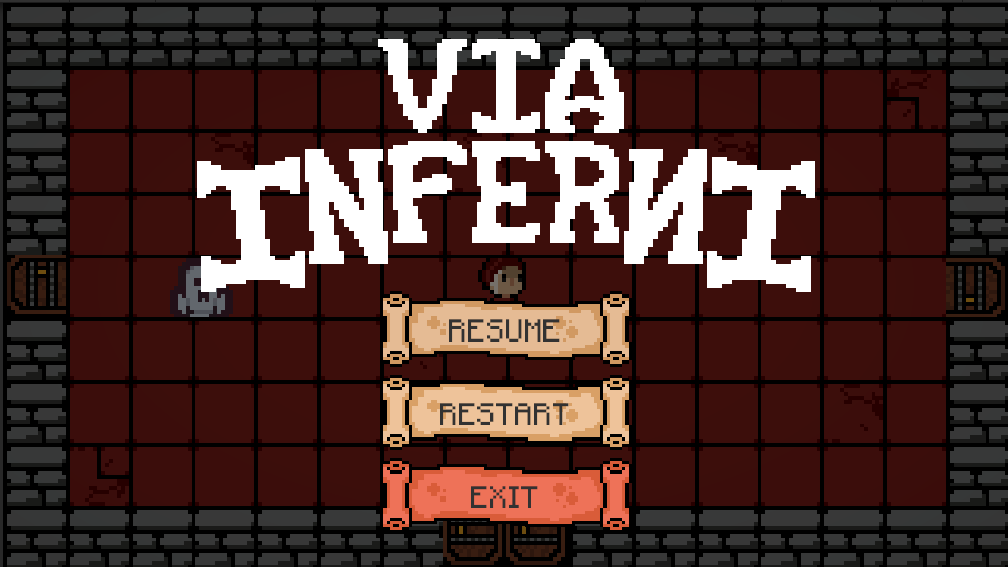
\includegraphics[width=.9\textwidth]{figures/resultados/iteracion4/11_menus_pausa.png}
\caption{Resultado de la feature Menú de Pausa en la iteración 4}
\label{fig:iteracion4-feature-menu-pausa}
\end{center}
\end{figure}

\subsection{Implementación de Menú Principal}
La implementación del menú principal se apoyó en \texttt{MainMenuController}, encargado de
vincular los botones principales con acciones como cargar la escena de juego o salir de la
aplicación. Esta separación permitió mantener el flujo de entrada al juego independiente de
la lógica de pausa usada durante la partida.

La parte final de la feature se completó con ajustes en la composición visual de la
pantalla, especialmente sobre el logotipo y la distribución de los botones, para que su
encaje fuera más consistente y adaptable.

\begin{figure}[htbp]
\begin{center}
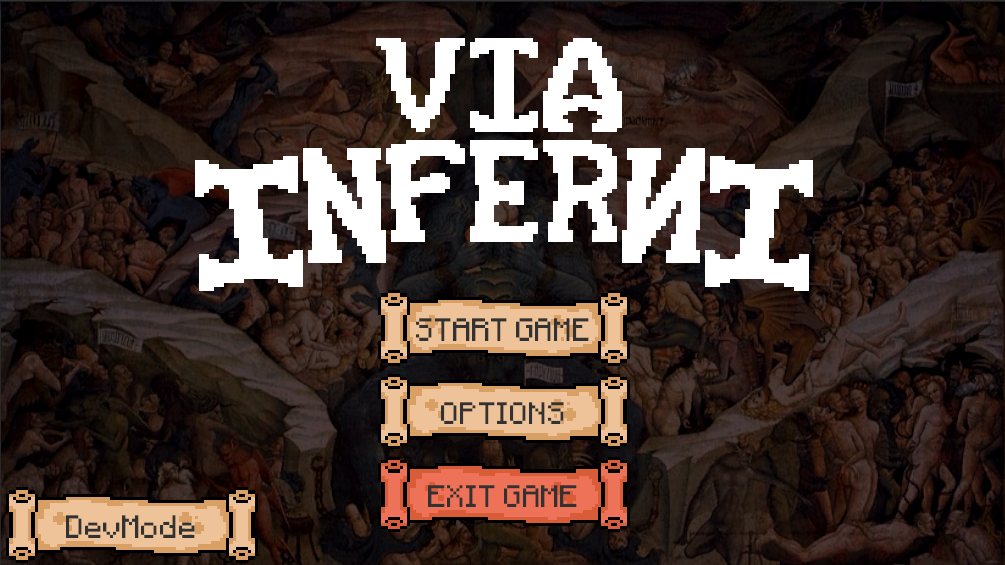
\includegraphics[width=.9\textwidth]{figures/resultados/iteracion4/12_menus_principal.png}
\caption{Resultado de la feature Menú Principal en la iteración 4}
\label{fig:iteracion4-feature-menu-principal}
\end{center}
\end{figure}

\paragraph{Actualizar Sprites.}
La actualización de sprites se realizó mediante la inserción de los nuevos recursos gráficos
diseñados para el juego y la revisión de los prefabs afectados. Al no requerir lógica propia
ni un controlador específico, esta mejora se documenta como una intervención de integración
visual: sustituir recursos provisionales, ajustar referencias y dejar los objetos principales
alineados con una estética más característica del proyecto.

\begin{figure}[htbp]
\begin{center}
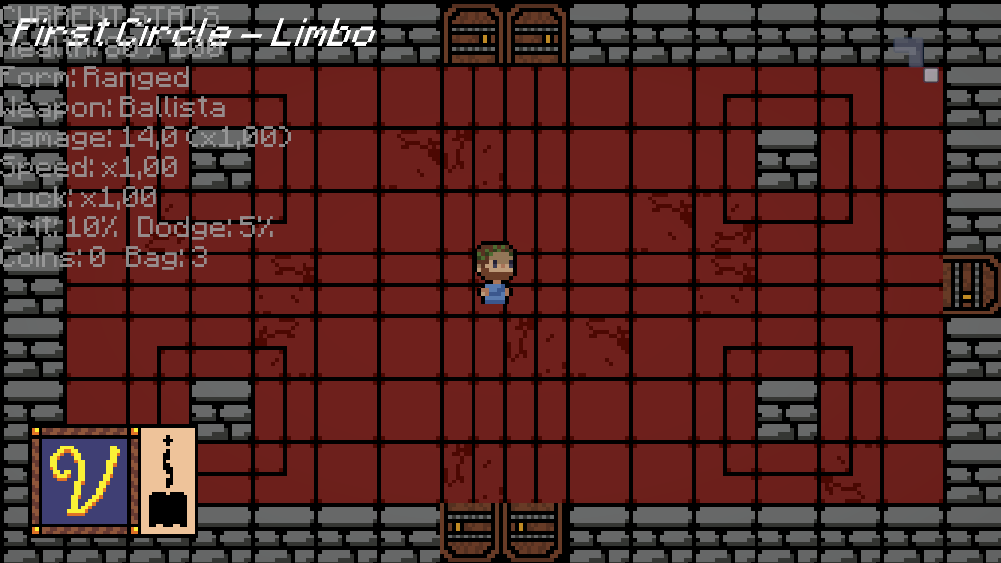
\includegraphics[width=.9\textwidth]{figures/resultados/iteracion4/13_actualizar_sprites.png}
\caption{Resultado de la feature Actualizar Sprites en la iteración 4}
\label{fig:iteracion4-feature-sprites}
\end{center}
\end{figure}

\section{Seguimiento y control}
El seguimiento de esta iteración mostró una relación bastante estable entre el alcance
previsto y el tiempo disponible. Las líneas de trabajo definidas, HUD, menú de pausa, menú
principal y actualización de sprites, pudieron desarrollarse dentro de la propia iteración y
no requirieron trasladar funcionalidades a entregas posteriores. El resultado fue una mejora
clara de la interacción con el sistema, de la legibilidad de la capa de presentación y de la
identidad visual del juego.

En términos de tiempo sí apareció una desviación moderada: frente a las 50:00 horas
planificadas, la iteración consumió 55:36 horas reales. Sin embargo, ese incremento no vino
acompañado de una ruptura del alcance, sino de un mayor esfuerzo de ajuste y consolidación en
una fase con menos incertidumbre técnica que otras anteriores.

Por ello, desde la perspectiva de seguimiento y control, esta iteración no exigió una
replanificación funcional relevante. Lo que se observa es más bien una sobrecarga moderada de
esfuerzo para cerrar con mayor consistencia la experiencia de usuario. La separación entre
menú de pausa y menú principal respondió a criterios de trazabilidad del trabajo y no a una
fragmentación forzada por falta de tiempo.

\begin{table}[h!]
    \centering
    \begin{coolTable}{p{.27\textwidth}p{.62\textwidth}}{2}
    {Pruebas de playtest realizadas en la iteración 4}
    \textbf{Feature bajo Test} & \textbf{Descripción de la prueba realizada} \\
    \midrule
    Head-Up Display & \begin{minipage}[t]{\linewidth}\begin{enumerate}\item Iniciar una partida y recorrer varias salas con combate y exploración. \item Observar la información visible del HUD durante el movimiento y los encuentros. \item Verificar que los elementos son legibles, no invaden de forma excesiva el área jugable y mantienen una proporción adecuada.\end{enumerate}\end{minipage} \\
    \midrule
    Menú de Pausa & \begin{minipage}[t]{\linewidth}\begin{enumerate}\item Abrir el menú de pausa durante la partida con teclado o mando. \item Probar las acciones de reanudar, reiniciar y salir. \item Confirmar que el tiempo de juego y el audio se detienen durante la pausa, que el HUD se oculta cuando corresponde y que la partida recupera su estado al reanudar.\end{enumerate}\end{minipage} \\
    \midrule
    Menú Principal & \begin{minipage}[t]{\linewidth}\begin{enumerate}\item Ejecutar el juego desde la escena de menú principal. \item Activar la opción de iniciar partida y volver posteriormente al menú. \item Comprobar que la escena de juego carga correctamente, que los botones responden y que la composición del logotipo y las acciones se mantiene estable.\end{enumerate}\end{minipage} \\
    \midrule
    Actualizar Sprites & \begin{minipage}[t]{\linewidth}\begin{enumerate}\item Recorrer una partida con los nuevos recursos visuales integrados. \item Observar jugador, elementos principales, interfaz y prefabs modificados. \item Verificar que los sprites aparecen correctamente referenciados, sin recursos provisionales visibles ni desajustes evidentes de escala o posición.\end{enumerate}\end{minipage} \\
    \end{coolTable}
    \caption{Pruebas de playtest realizadas en la iteración 4.}
\end{table}

\begin{table}[h!]
    \centering
    \begin{coolTable}{lr}{2}
    {Horas de la iteración 4}
    \textbf{Horas planificadas de la iteración} & 50:00 \\
    \textbf{Horas reales (Adolfo Borrego González)} & 31:04 \\
    \textbf{Horas reales (Germán Sánchez Carmona)} & 24:32 \\
    \textbf{Horas reales totales de la iteración} & 55:36 \\
    \textbf{Horas acumuladas planificadas hasta esta iteración} & 300:00 \\
    \textbf{Horas acumuladas reales hasta esta iteración} & 303:30 \\
    \end{coolTable}
    \caption{Resumen de horas reales de la iteración 4.}
\end{table}

\begin{figure}[htbp]
\begin{center}
% \missingfigure{Sustituir por el diagrama UML de resultado de la iteración 4}
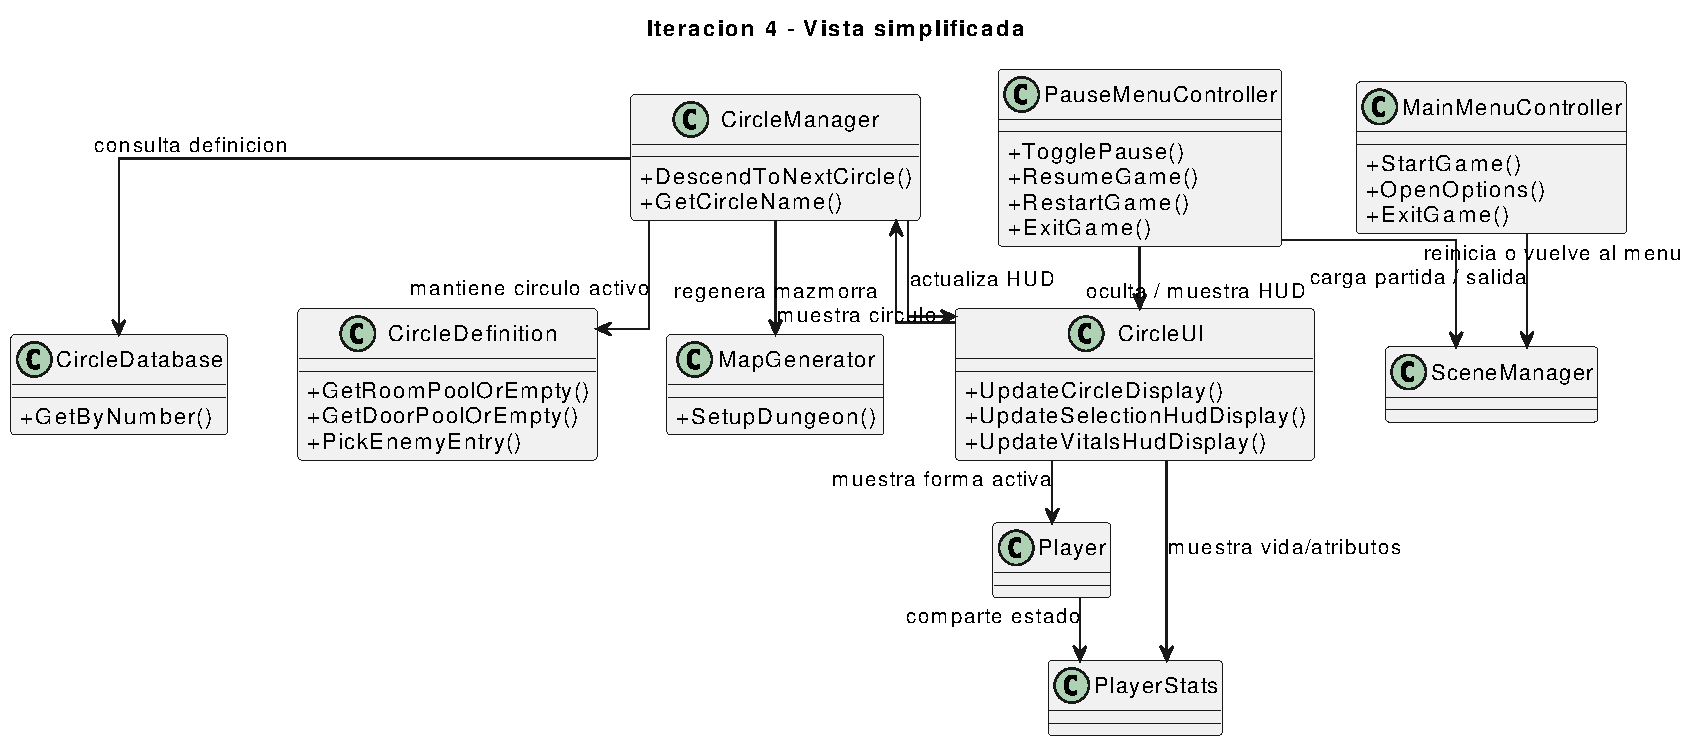
\includegraphics[width=\textwidth]{figures/iteracion4_resultado_uml.pdf}
\caption{Diagrama UML de resultado de la iteración 4}
\label{fig:uml-resultado-iteracion4}
\end{center}
\end{figure}
